\documentclass[]{subfiles}

\begin{document}
\section{Zeitauswertung}
Für die Studienarbeit werden pro Person 8 ECTS angerechnet.
Dies entspricht insgesamt 480 Stunden Aufwand für die Studienarbeit oder 
jeweils 240 Stunden pro Person.
Auf 15 Wochen Projektdauer fallen somit pro Woche 16 Stunden für die Projektarbeit an.

\subsection{Zeitauswertung Mike Schmid}
\begin{figure}[h!]
    \begin{center}
        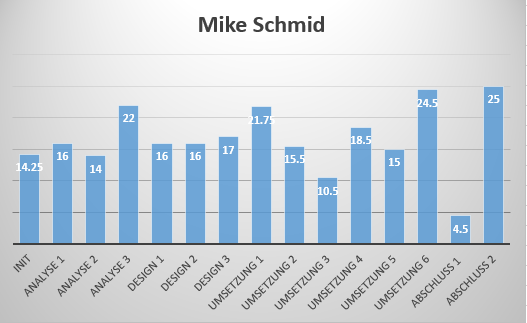
\includegraphics[scale=0.75]{\vorlagenOrdner/Bilder/Zeitanalyse/zeit_mike_schmid}
    \end{center}
    \caption{Zeitanalyse Mike Schmid}
\end{figure}

\subsection{Zeitauswertung Janik Schlatter}
\begin{figure}[h!]
    \begin{center}
        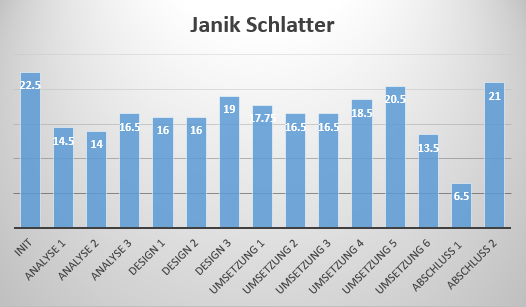
\includegraphics[scale=0.75]{\vorlagenOrdner/Bilder/Zeitanalyse/zeit_janik_schlatter}
    \end{center}
    \caption{Zeitanalyse Janik Schlatter}
\end{figure}

\newpage

\subsection{Zeitauswertung Projekt}
\begin{figure}[h!]
    \begin{center}
        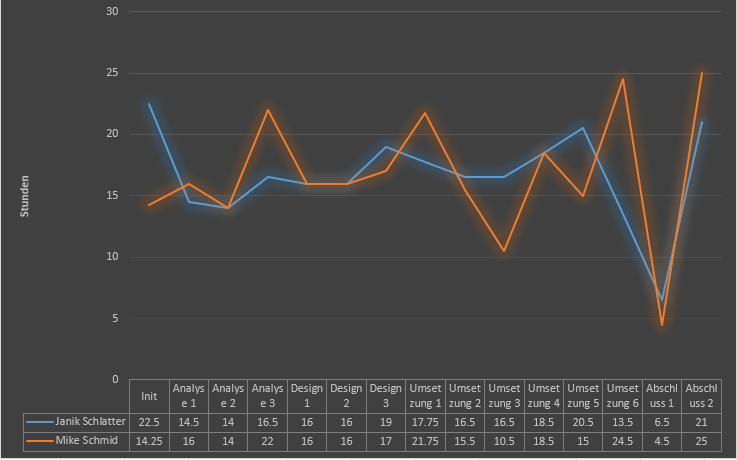
\includegraphics[scale=0.9]{\vorlagenOrdner/Bilder/Zeitanalyse/zeit_gemeinsam}
    \end{center}
    \caption{Zeitanalyse Projekt}
\end{figure}
\end{document}

Mit einer gemeinsamen totalen Projektzeit von 499.75 Stunden wurden die vorgegebenen
480 Stunden mit 19.75 Stunden überschritten.
Diese Abweichung von ca 4\% von der vorgegebenen Projektdauer lässt sich mit der
Nachbearbeitung der Anforderungsanalyse und mit einer kurzen Umstellungsphase 
aufgrund des Covid-19 Virus erklären und lieg absolut innerhalb der Toleranzgrenzen.